\mchapter{شرح مسئله}
در \CurrentProject قصد داریم در یک سامانه‌ی رایانش لبه‌ای مطابق با شکل \ref{fig-offloading-system}، استراتژی تخلیه‌ای بیابیم که تاخیر سرویس میانگین $\bar{T}$ را تحت محدودیت توان مصرفی $P_{m a x}$ در درازمدت کمینه کند.
\begin{figure}[H]
	\centering
	\includegraphics*[width=\textwidth]{figures/MEC5.png}
	\caption{ساختار کلی سامانه‌ی تخلیه‌ی پردازش}
	\label{fig-offloading-system}
\end{figure}
\newpage
همانطور که در شکل \ref{fig-offloading-system} مشاهده می‌شود، در سامانه مد نظر سه مولفه اصلی وجود دارد:
\begin{enumerate}
	\item دستگاه کاربر (\lr{User Equipment})
	\item سرور رایانش لبه‌ای چند-دسترسی (\lr{Multi-access Edge Computing Server})
	\item کانال بیسیم
\end{enumerate}
در فصل جاری نحوه‌ی عملکرد هر کدام از این مولفه‌ها در قالب مدل‌های تئوری شرح داده می‌شود.

\section{مدل وظایف}
فرض می‌شود که \(k\) نوع وظیفه‌ی مختلف در سیستم رایانش لبه‌ای وجود دارد و به ازای هر نوع وظیفه دقیقا یک صف در سیستم وجود دارد. وظایف نوع \(i\)-اُم برای اجرا به صورت محلی\LTRfootnote{Local} احتیاج به \(L_i\) بازه زمانی پردازش توسط پردازنده دارند و به منظور تخلیه به سرور رایانش لبه‌ای احتیاج به \(M_i\) واحد زمانی ارسال توسط واحد ارسال\LTRfootnote{Transmission Unit} دارند. همچنین فرض می‌شود که وظایف نوع \(i\)-اُم در سرور رایانش لبه‌ای به \(C_i\) بازه زمانی پردازش توسط سرور نیاز دارند. برای سادگی بیشتر در ادامه‌ی \CurrentProject برای اشاره به یک واحد زمانی اجرا توسط پردازنده از عبارت \textbf{«قسمت»}\LTRfootnote{Section} استفاده می‌کنیم که انتزاعی از قسمت‌های کد اجرایی است. و برای اشاره به یک واحد زمانی ارسال توسط واحد ارسال از عبارت\textbf{ «بسته» }استفاده می‌شود.
\newpage
\section{مدل دستگاه کاربر}
\label{sec:ue-model}
دستگاه کاربر مطابق با شکل \ref{fig-offloading-system} شامل دو مولفه‌ی پردازنده و واحد ارسال می‌باشد. همچنین همانطور که اشاره شد \(k\) صف مختلف به ازای هر کدام از انواع وظایف در سیستم وجود دارد. ظرفیت هر صف را برابر با مقدار ثابت \(Q\) در نظر می‌گیریم. \\

در هر بازه زمانی، پردازنده یا به اندازه‌ی یک قسمت پردازش انجام می‌دهد و یا بیکار\LTRfootnote{Idle} است. اجرای هر قسمت پردازش توسط پردازنده به میزان
\(P_{l o c}\)
وات توان مصرف می‌کند. به طور مشابه واحد ارسال در هر بازه زمانی یا یک بسته را به شبکه ارسال می‌کند یا بیکار است. نکته قابل توجه در مورد واحد ارسال این است که با توجه به شرایط کانال بیسیم، در یک بازه زمانی خاص ممکن است ارسال موفقیت آمیز باشد یا نباشد. فرض می‌شود که ارسال موفقیت آمیز هر بسته به میزان
\(P_{t x}\)
وات توان مصرف می‌کند. توضیحات بیشتر در مورد نحوه‌ی کارکرد کانال بی‌سیم در بخش \ref{sec:wireless} آورده شده است. \\

با توجه به توضیحات داده شده می‌توان مدلی برای «حالت دستگاه کاربر»\LTRfootnote{User Equipment State} تعریف کرد. در \cite{Liu} برای مشخص کردن حالت دستگاه در زمان \(t\) از یک سه تایی مانند $\boldsymbol{\tau}[t]=\left(q[t], c_{T}[t], c_{L}[t]\right)$ استفاده شده است، که در آن \(q[t]\) مشخص کننده تعداد وظایف موجود در صف وظایف، \(c_T[t]\) مشخص کننده تعداد بسته ارسال شده از وظیفه‌ی تخصیص داده شده به واحد ارسال است، و \(c_L[t]\) مشخص کننده تعداد قسمت اجرا شده از وظیفه تخصیص داده شده به پردازنده است. همچنین حالت \(c_T[t] = 0\) معادل با بیکار بودن واحد ارسال و \(c_L[t] = 0\) معادل با بیکار بودن پردازنده تعریف می‌شود. برای مثال سه تایی \((4, 2, 1)\) به این معنی است که ۴ وظیفه در صف وظایف وجود دارد، واحد پردازش در حال تخلیه‌ی وظیفه‌ای است و تا کنون یک بسته از آن وظیفه را ارسال کرده و به عنوان قدم بعدی باید بسته شماره ۲ را ارسال کند. پردازنده نیز در حال اجرای وظیفه‌ای به صورت محلی است و تا کنون یک قسمت از آن وظیفه را اجرا کرده است. \\
\newpage
با این حال مدل فوق در مسئله‌ی تخلیه‌ی وظیفه‌ی با چند نوع وظیفه، قابل استفاده نیست و نیاز به تغییر دارد. ما در \CurrentProject برای تعیین حالت دستگاه کاربر از یک چندتایی\LTRfootnote{Tuple} به طول \(k + 4\) مطابق با رابطه‌ی \ref{eg:state} استفاده می‌کنیم. در این رابطه‌ی متغیرهای
\(q_1[t], \cdots, q_k[t]\)
تعداد وظایف موجود از هر نوع وظیفه در صف مربوطه را مشخص می‌کنند. متغیرهای \(c_R[t]\) و \(c_L[t]\) مشابه با حالت تک صف تعریف می‌شوند و به ترتیب وضعیت واحد ارسال و پردازنده را مشخص می‌کنند. دو متغیر جدید \(T_R[t]\) و \(T_L[t]\) به ترتیب مشخص کننده نوع وظیفه در حال ارسال توسط واحد ارسال و نوع وظیفه در حال اجرا توسط پردازنده اند.
\begin{equation}
	\label{eg:state}
	\tau[t]=\left(q_{1}[t], q_{2}[t], \ldots, q_{k}[t], c_{R}[t], c_{L}[t], T_{R}[t], T_{L}[t]\right)
\end{equation}
در \CurrentProject به منظور خوانایی بیشتر، چندتایی بیان شده در رابطه‌ی \ref{eg:state} را به صورت زیر نیز نمایش می‌دهیم و این دو صورت معادل هم می‌باشند:
\begin{equation}
	\label{eg:state2}
	\tau[t]=\left([q_{1}[t], q_{2}[t], \ldots, q_{k}[t]], c_{R}[t], c_{L}[t], T_{R}[t], T_{L}[t]\right)
\end{equation}
رابطه‌ی \ref{eq:state-space} با تعریف شروط مختلف فضای حالت مسئله را توصیف می‌کند. \textbf{(نکته: در رابطه‌ی \ref{eq:state-space} و سراسر \CurrentProject منظور از \(\tau\{X\}\) مقدار متغیر \(X\) در حالت \(\tau\) است.)}
\begin{equation}
	\label{eq:state-space}
	\begin{aligned}
		&\forall \tau \in S, i \in \{1,2, \ldots, k\} \quad 0 \leqslant\tau\left\{q_{i}\right\} \leqslant Q\\
		&\forall \tau \in S \quad  \tau\left\{T_L\right\},  \tau\left\{T_R\right\} \in \{0, 1,2, \ldots, k\}\\
		&\left.\forall \tau \in\left\{\tau^{\prime} \in S \mid \tau^{\prime}\left\{T_{R}\right\}=0\right\} \quad \tau\{C_R\right\}=0\\
		&\forall \tau \in\left\{\tau^{\prime} \in S \mid \tau^{\prime}\left\{T_{R}\right\} \neq 0\right\} \quad 1 \leqslant \tau\left\{C_{R}\right\} \leqslant M_{\tau\{T_{R}\}} \\
		&\left.\forall \tau \in\left\{\tau^{\prime} \in S \mid \tau^{\prime}\left\{T_{L}\right\}=0\right\} \quad \tau\{C_L\right\}=0\\
		&\forall \tau \in\left\{\tau^{\prime} \in S \mid \tau^{\prime}\left\{T_{L}\right\} \neq 0\right\} \quad 1 \leqslant \tau\left\{C_{L}\right\} \leqslant L_{\tau\{T_{L}\}} - 1
	\end{aligned}
\end{equation}

\newpage
\section{مدل زمان}
وضعیت سیستم تخلیه‌ی وظیفه در فواصل زمانی\LTRfootnote{Time Slot} با طول ثابت \(\Delta\) میلی ثانیه بررسی می‌شود. برای مثال حالت دستگاه کاربر را در بازه زمانی \(t\)-اُم با \(\tau[t]\) مشخص می‌کنیم، و حالت دستگاه در بازه زمانی \(t + 1\) را با \(\tau[t + 1]\) مشخص می‌کنیم و فاصله بین این دو بازه زمانی \(\Delta\) میلی ثانیه است. \\

بررسی زمان به صورت واحدهای گسسته به منظور ساده‌سازی مسئله و همچنین گسترش پذیری آن به شرایط محیطی مختلف صورت گرفته است. در عمل، یک مقدار قابل استفاده برای \(\Delta\) طول بازه‌های زمانی شبکه‌ی دسترسی\LTRfootnote{Access Network} مورد نظر است. برای مثال در شبکه‌های \lr{LTE} طول هر بازه زمانی ۵/۰ میلی‌ثانیه می‌باشد. \cite{LTE}

\section{مدل کانال بیسیم}
\label{sec:wireless}
در \CurrentProject مشابه با \cite{Liu} کانال بی‌سیم را به صورت تصادفی مدل می‌کنیم\LTRfootnote{Stochastic Channel} یکی از دلایل اصلی برای مدل‌سازی کانال به صورت تصادفی، وجود نویز و ناپایداری در ارتباطات بیسیم است. کانال بی‌سیم را با یک مدل ساده احتمالی دوجمله‌ای  مدل می‌کنیم به این صورت که ارسال هر بسته توسط واحد ارسال با احتمال \(\beta\) موفقیت آمیز خواهد بود و با احتمال \(1 - \beta\) ناموفق خواهد بود. در عمل مقدار \(\beta\) با توجه به رابطه‌ی \ref{eq:shannon} (رابطه‌ی شنون) محاسبه می‌شود، که در آن \(R\) مشخص کننده سایز هر بسته است،
$r(t)$
مشخص کننده‌ی نرخ ارسال در زمان
$t$
،
 \(B\) پهنای باند سیستم، \(\gamma[t]\) مقدار بهره‌ی کانال\LTRfootnote{Channel Gain} و \(N_0\) مشخص کننده اندازه‌ی نویز کانال است.
\begin{equation}
	\label{eq:shannon}
	\begin{aligned}
		&\beta=P(r(t) \geq R) \\
		&r(t)=B \log _{r}\left(1+\frac{\gamma[t] P_{\mathrm{tx}}}{N_0 B}\right)
	\end{aligned}
\end{equation}
\section{مفهوم کنش}
\label{sec:action}
یک استراتژی تخلیه در هر بازه زمانی مانند \(t\) می‌بایست یک کنش\LTRfootnote{Action} مانند \(v[t]\) را برای اجرا توسط دستگاه کاربر انتخاب کند. اجرای هر کنش می‌تواند حالت دستگاه کاربر را تغییر دهد. برای درک بهتر مفهوم کنش، ابتدا مشابه \cite{Liu} حالتی را در نظر می‌گیریم که تنها یک صف (یک نوع وظیفه) در سیستم وجود داشته باشد. در این حالت می‌توانیم مجموعه‌ی کنش‌ها را با چهار عضو مطابق جدول \ref{table:actions} مشخص کنیم.

\begin{table}[H]
	\centering
	\begin{latin}
		\begin{tabular}{@{}lrll@{}}
			\toprule
			\textbf{ID} & \textbf{Transmit} & \textbf{Local Execution} & \textbf{Description} \\ \midrule
			1           & False             & False                    & No operation         \\
			2           & False             & True                     & Add to CPU           \\
			3           & True              & False                    & Add to TU            \\
			4           & True              & True                     & Add to both units    \\ \bottomrule
		\end{tabular}
	\end{latin}
	\caption{لیست کنش‌ها در سیستمی با یک صف وظیفه}
	\label{table:actions}
\end{table}
به طور مشابه در شرایطی که بیش از یک نوع وظیفه در سیستم وجود داشته باشد مجموعه‌ی کنش‌های ممکن مطابق با جدول \ref{table:actions-multiqueue} بدست می‌آید.
\begin{table}[H]
	\centering
	\begin{latin}
		\begin{tabular}{@{}lrlll@{}}
			\toprule
			\textbf{ID}                     & \textbf{Transmit} & \textbf{Local Execution} & \textbf{Description} & \textbf{Count}                \\ \midrule
			$\{1\}$                           & False             & False                    & No operation         & 1                    \\
			$\{2, ..., k + 1\}$               & False             & True                     & Add to CPU           & $k$                    \\
			$\{k + 2, ..., 2k + 1\}$          & True              & False                    & Add to TU            & $k$                    \\
			$\{2k + 2, ..., 2k + k * k - 1\}$ & True              & True                     & Add to both units    & $k^2$ \\ \bottomrule
		\end{tabular}
	\end{latin}
	\caption{تقسیم‌بندی کنش‌ها در سیستمی با $k$ صف وظیفه}
	\label{table:actions-multiqueue}
\end{table}
اجرای هر کنش طبعا ممکن است که حالت سیستم را تغییر دهد. به طور مثال اجرای هر کنش نوع \lr{Add To CPU} یک وظیفه را از صف مربوطه بر می‌دارد، بنابراین طول صف مطابق (\(q_i[t + 1] = q_i[t] - 1\) تغییر می‌کند. با اجرای این کنش همچنین وضعیت پردازنده از \(c_L[t] = 0\) یعنی حالت بیکار به \(c_L[t + 1] = 1\) تغییر خواهد کرد زیرا قسمت اول وظیفه مربوطه در بازه زمانی \(t\) انجام خواهد شد. به طور مشابه برای سایر کنش‌ها نیز میتوان توابع انتقال\LTRfootnote{Transition Function} مشخص تعریف کرد که با گرفتن یک حالت ورودی، حالت خروجی را محاسبه نماید. به دلیل پیچیدگی روابط این توابع، از توضیح بیشتر در این بخش صرف نظر شده است. برای مشاهده منطق دقیق این توابع در قالب کد، به پیوست ۱ مراجعه شود.
\section{استراتژی تخلیه‌ی وظیفه}
استراتژی تخلیه‌ی وظیفه در هر بازه زمانی تصمیم می‌گیرد که دستگاه کاربر چه کنشی را اجرا کند. بنابراین استراتژی تخلیه یک تابع مانند $G(\tau)$ می‌باشد که با گرفتن حالت دستگاه کاربر $\tau[t]$ به عنوان ورودی، یک کنش مانند \(a\) را به عنوان خروجی می‌دهد. لازم به ذکر است که در اینجا این تابع را به صورت مفهومی انتزاعی در نظر می‌گیریم و در فصل‌های آتی به طور دقیق به نحوه‌ی بدست آوردن تابع بهینه $g(\tau)^{*}$ می‌پردازیم.
\newpage
\section{روند فعالیت سیستم تخلیه‌ی وظیفه}
نحوه‌ی عملکرد دستگاه کاربر در هر بازه زمانی مطابق با فرآیند مشخص شده در شکل \ref{fig:ueproc} می‌باشد. در هر باز، دستگاه کاربر ابتدا کنش اجرایی را از یک استراتژی تخلیه دریافت می‌کند. سپس کنش انتخاب شده توسط دستگاه کاربر اجرا خواهد شد که ممکن است منجر به تغییر حالت دستگاه شود. سپس پردازنده و واحد ارسال هر کدام در صورت فعال بودن به اندازه‌ی یک بازه زمانی فعالیت خواهند کرد. در انتها وظایف جدید با احتمالات
$\alpha_1, \cdots, \alpha_k$
به صف‌های وظایف اضافه خواهند شد.


\begin{figure}[H]
	\centering
	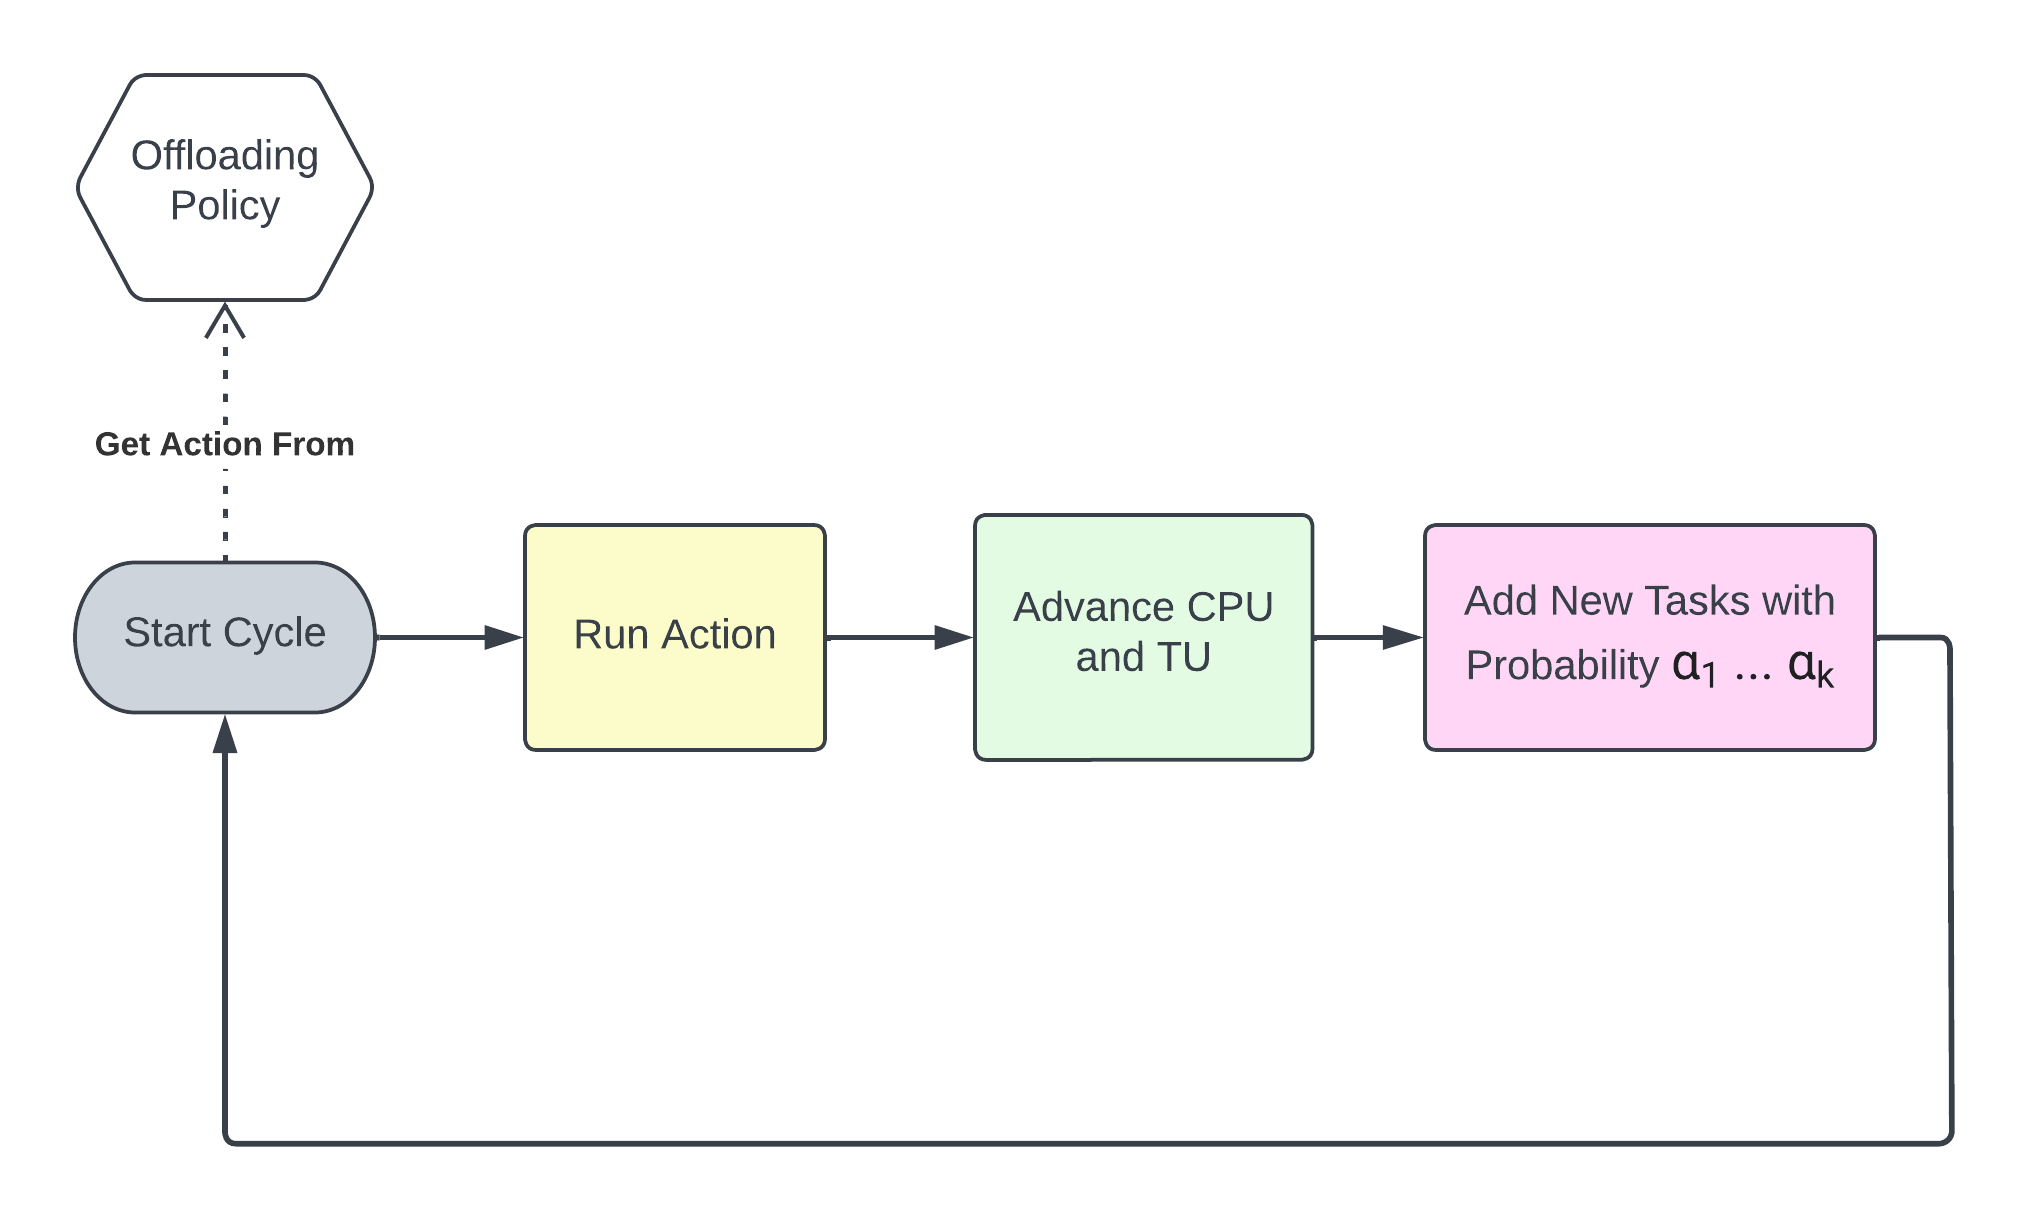
\includegraphics[width=\textwidth]{figures/ueproc.png}
	\caption{روند فعالیت دستگاه کاربر}
	\label{fig:ueproc}
\end{figure}